\begin{figure}[H]
\centering
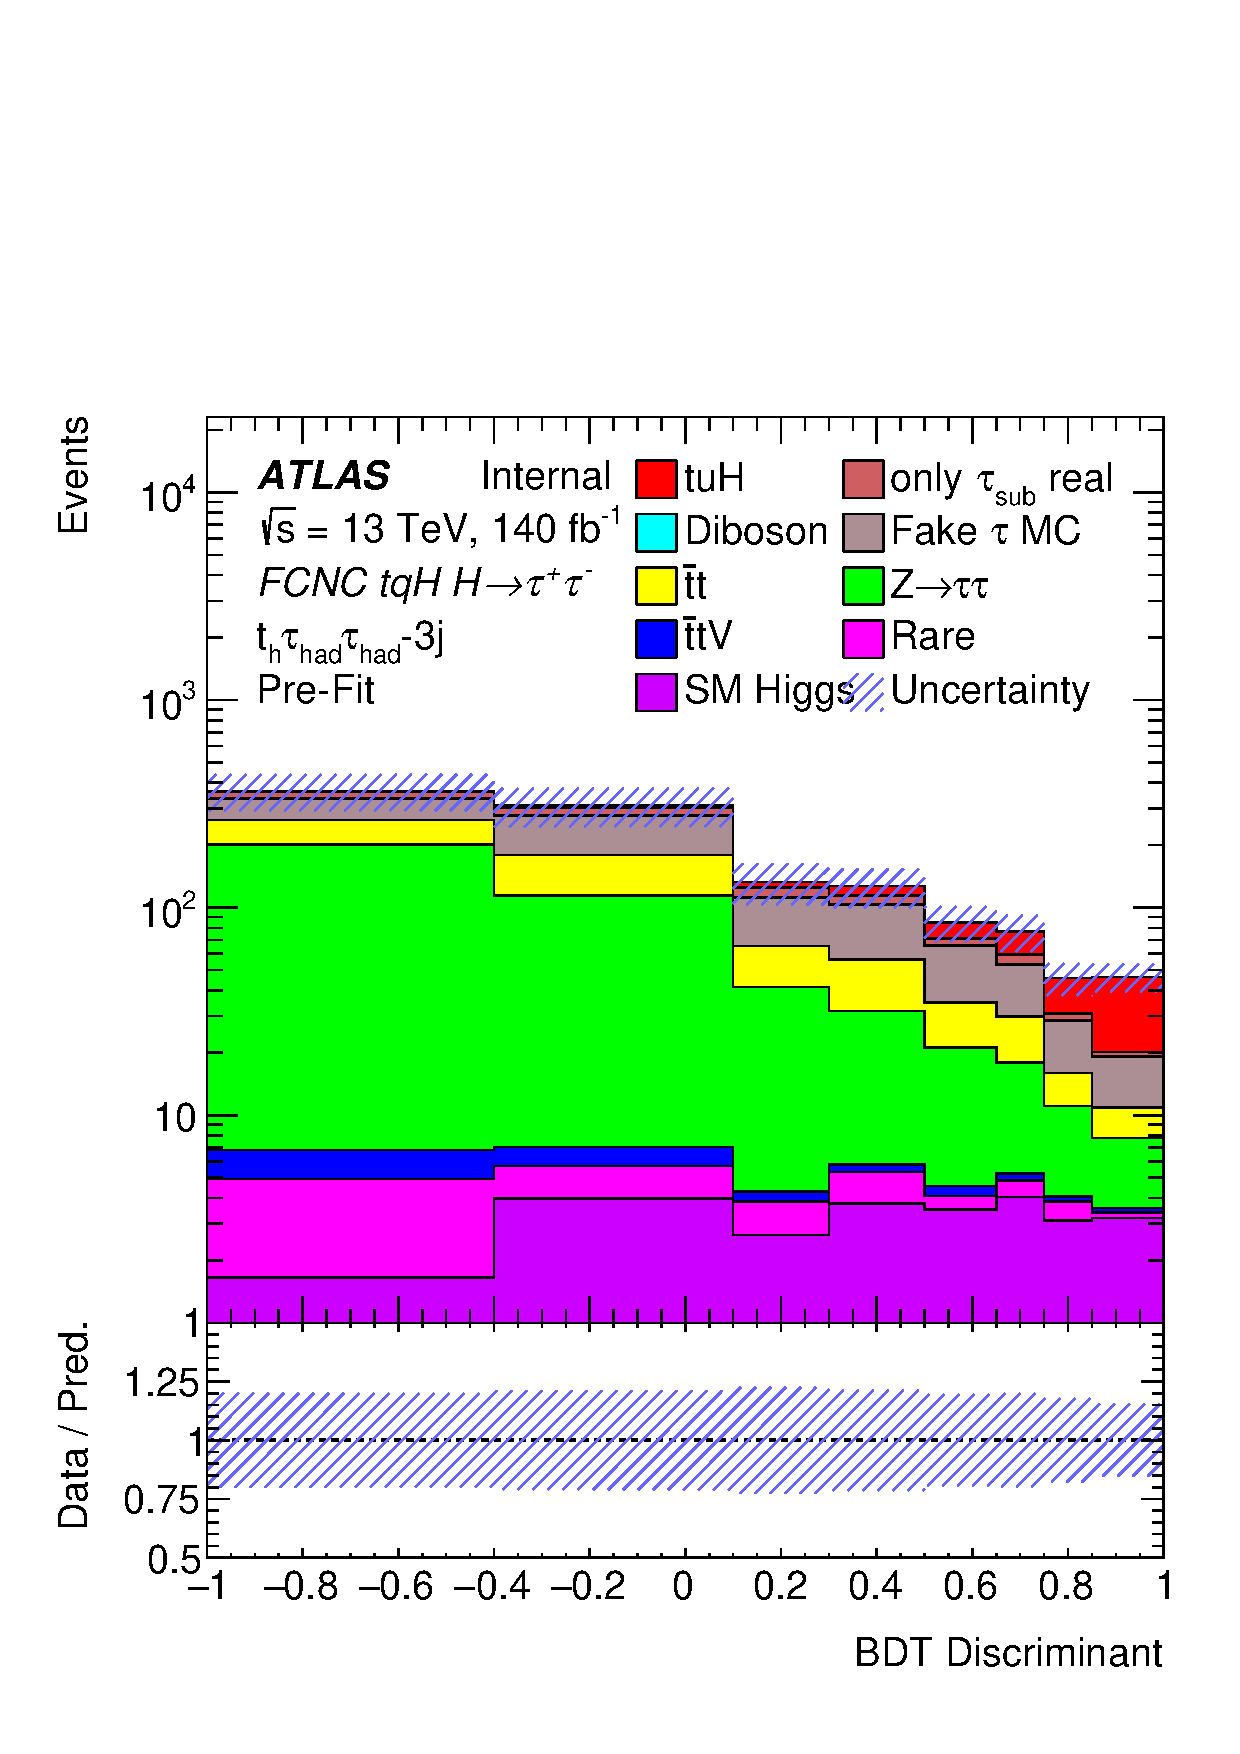
\includegraphics[width=0.30\textwidth]{\FCNCFigures/xTFW/Limit/tuH_reg2mtau1b3jos_vetobtagwp70_highmet.pdf}
\put(-100, 55){\textbf{(a1)}}
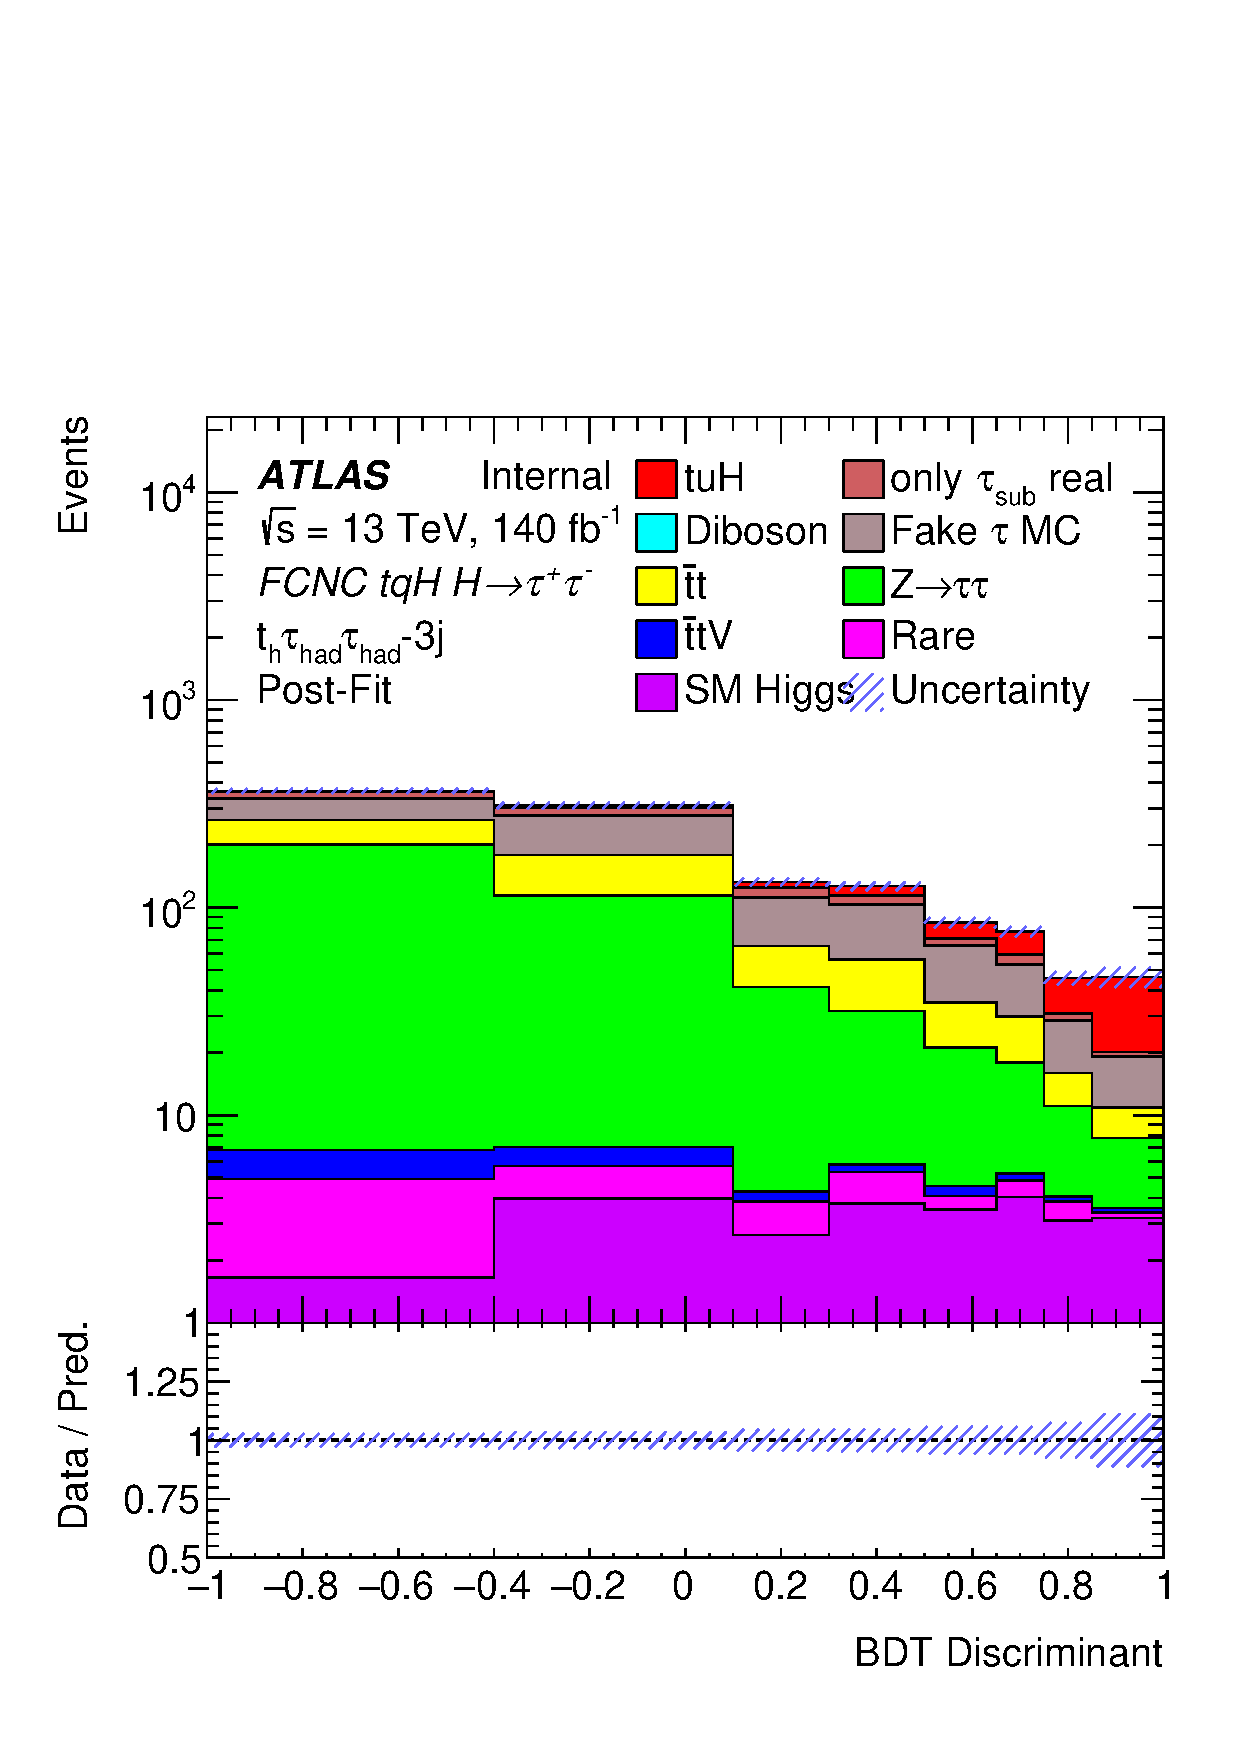
\includegraphics[width=0.30\textwidth]{\FCNCFigures/xTFW/Limit/tuH_reg2mtau1b3jos_vetobtagwp70_highmet_postFit.pdf}
\put(-100, 55){\textbf{(a2)}}
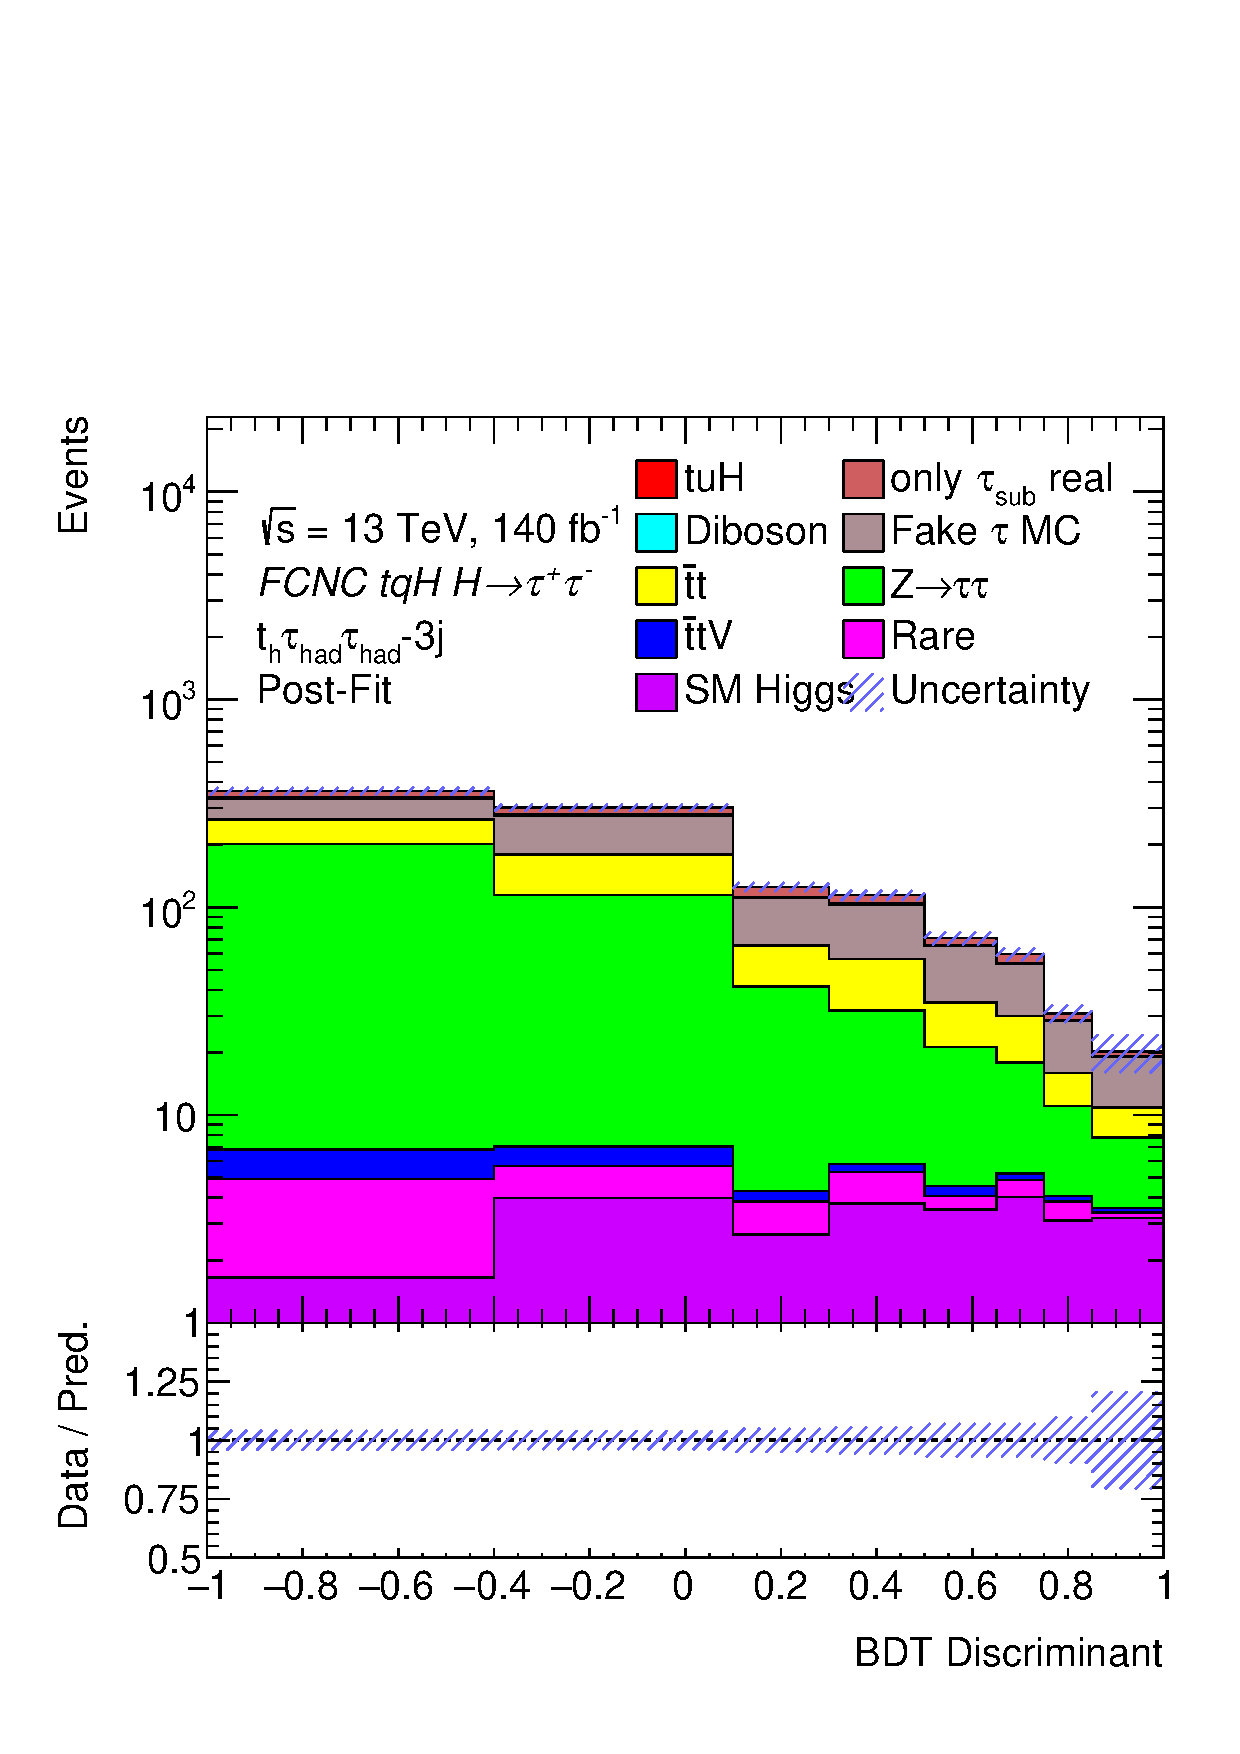
\includegraphics[width=0.30\textwidth]{\FCNCFigures/xTFW/Limit/tuH_reg2mtau1b3jos_vetobtagwp70_highmet_postFit_BOnly.pdf}
\put(-100, 55){\textbf{(a3)}}\\
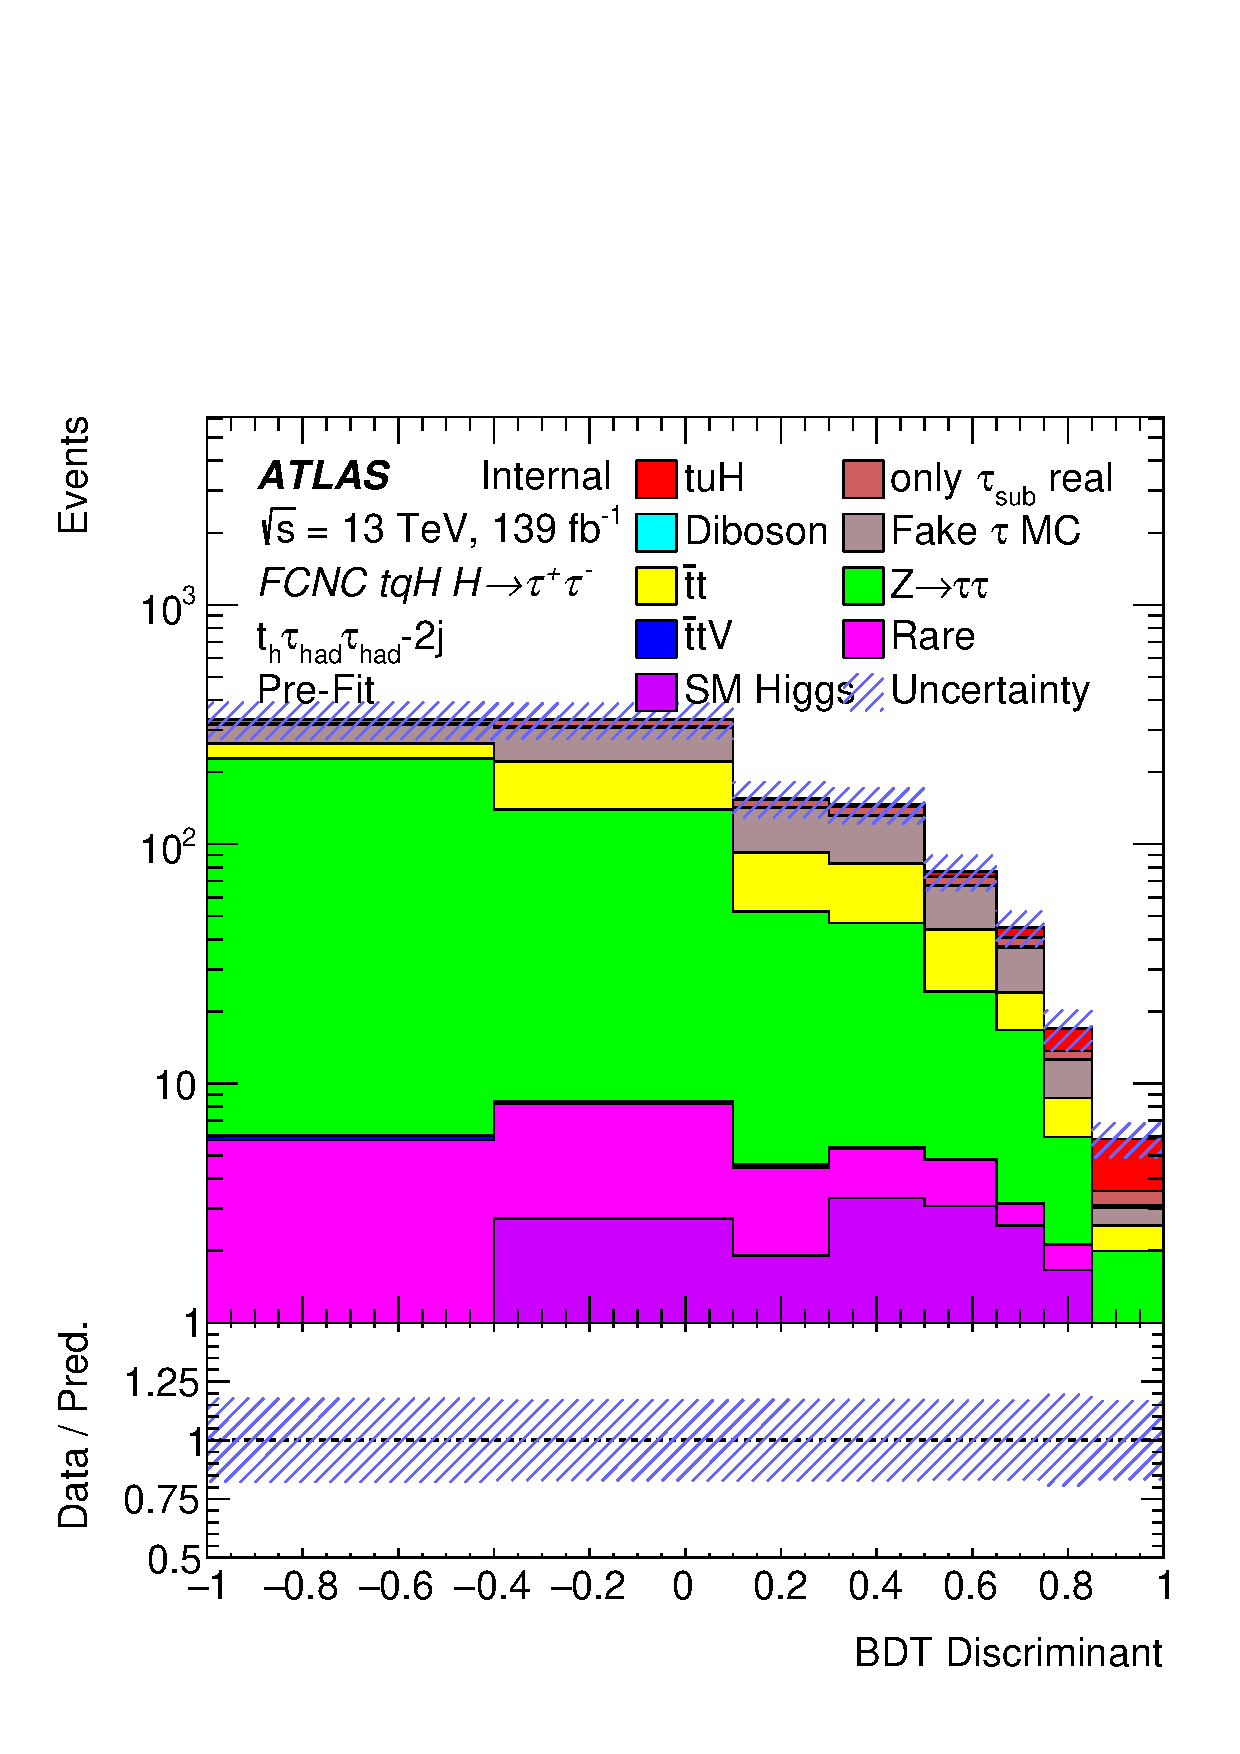
\includegraphics[width=0.30\textwidth]{\FCNCFigures/xTFW/Limit/tuH_reg2mtau1b2jos_vetobtagwp70_highmet.pdf}
\put(-100, 55){\textbf{(b1)}}
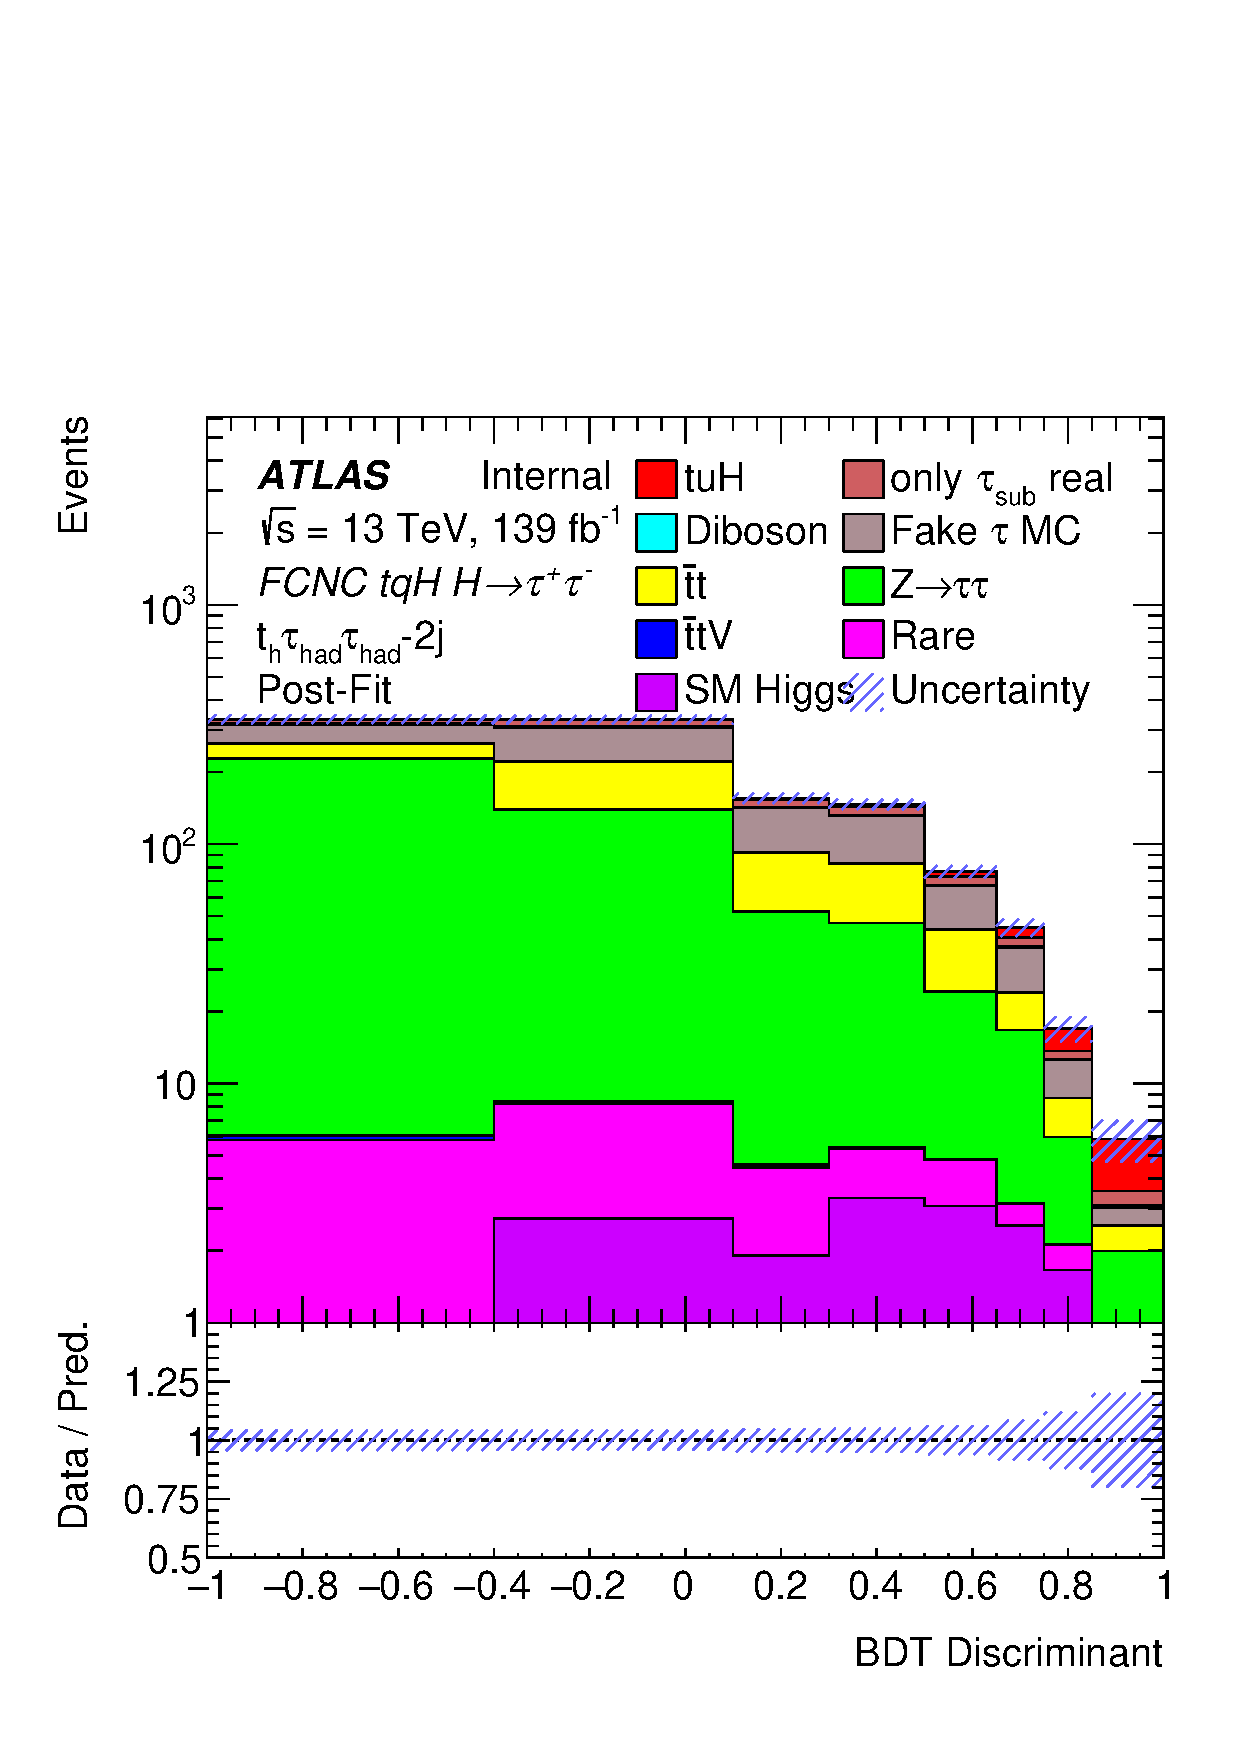
\includegraphics[width=0.30\textwidth]{\FCNCFigures/xTFW/Limit/tuH_reg2mtau1b2jos_vetobtagwp70_highmet_postFit.pdf}
\put(-100, 55){\textbf{(b2)}}
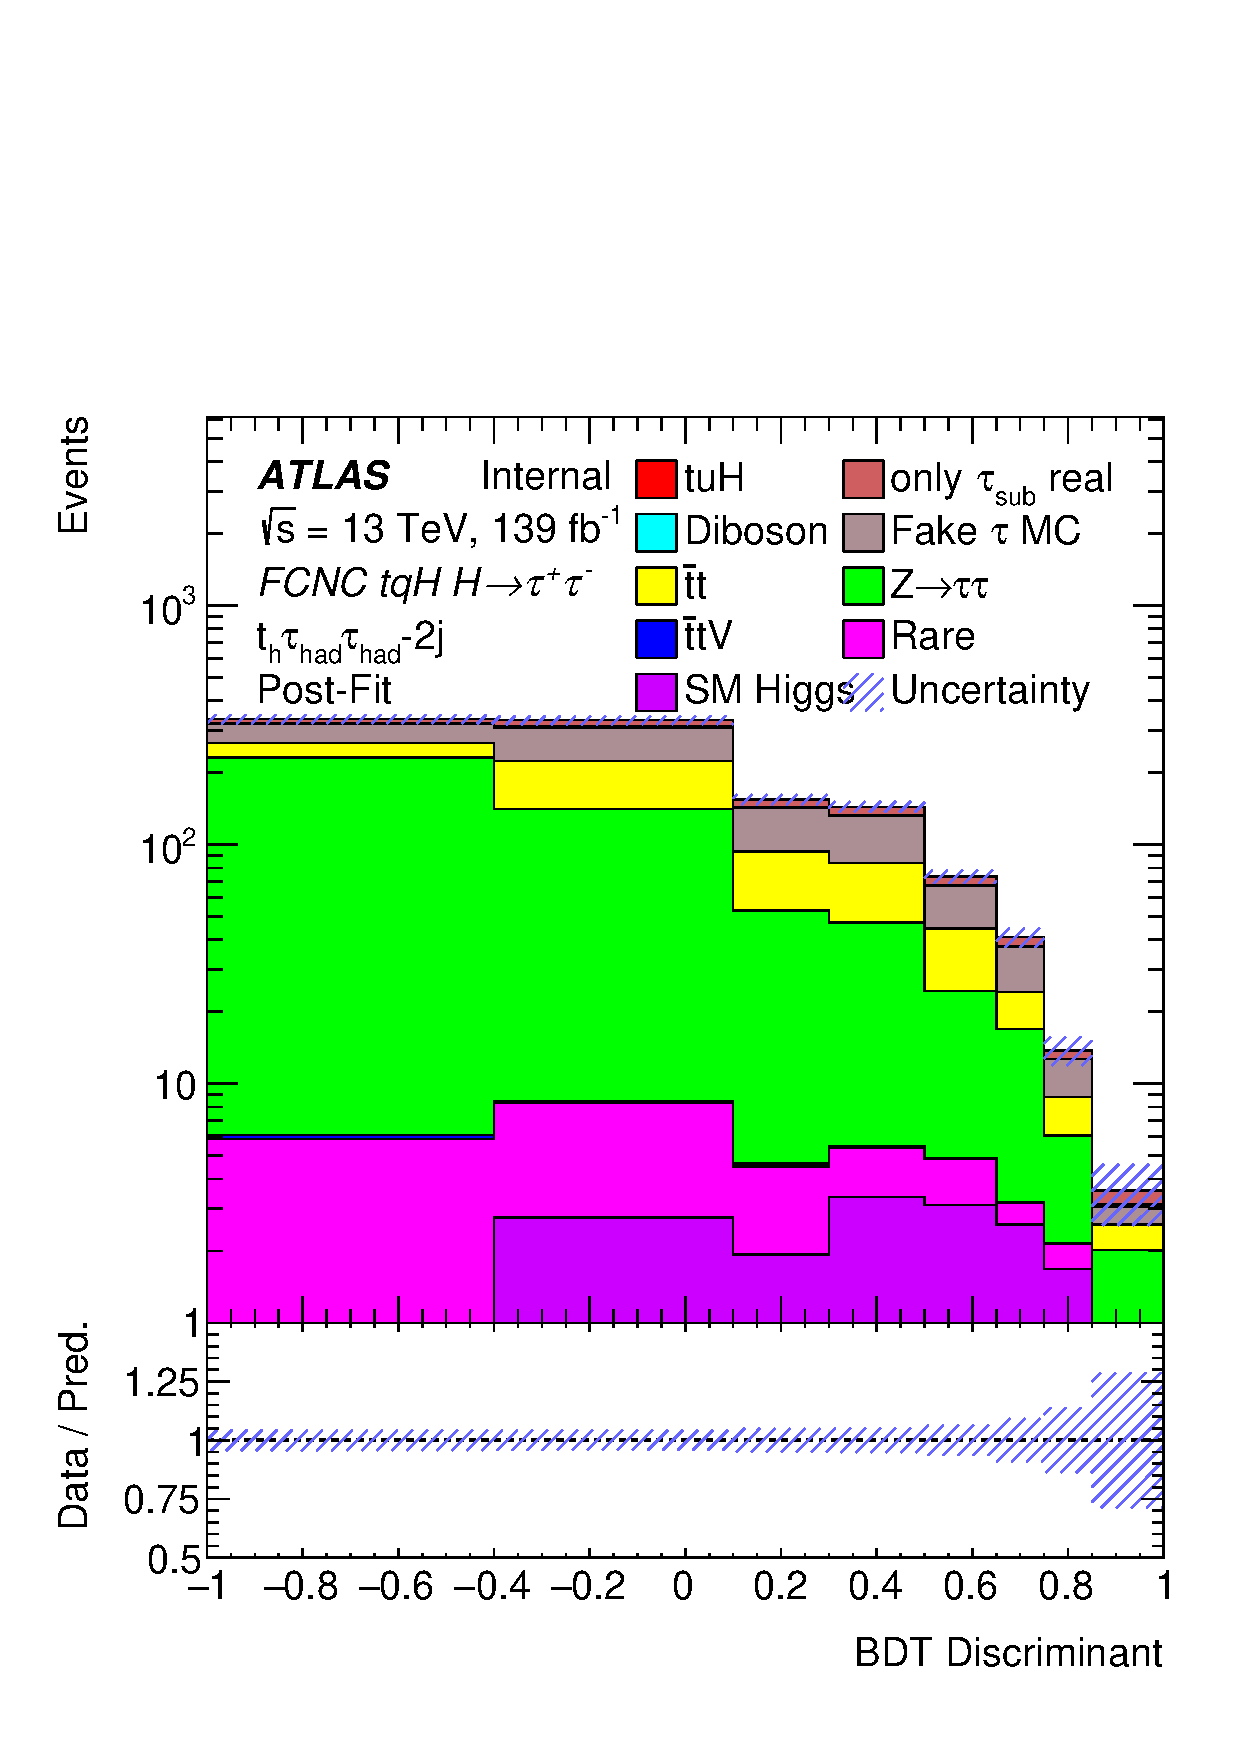
\includegraphics[width=0.30\textwidth]{\FCNCFigures/xTFW/Limit/tuH_reg2mtau1b2jos_vetobtagwp70_highmet_postFit_BOnly.pdf}
\put(-100, 55){\textbf{(b3)}}\\

%\caption{ The asimov prefit (left) and postfit (right) BDT distributions in the $t_h\thadhad$-3j (a1-2) and $t_h	hadhad$-2j (b1-2)}
%\label{fig:xTFW_trexPrefit}
%\end{figure}

\caption{ Comparison of the shape of the BDT discriminant distribution between the asimov prefit (a1,b1), asimov postfit  with $\mu$=1 (a2,b2) and background only fit (a3,b3). The upper three plots are in the  $t_h\thadhad$-3j (a1-a3) region, and the bottom three are in $t_h\thadhad$-2j (c1-c3). Statistical and systematic uncertainties are being shown.}
\label{fig:xTFW_trexPrefit}
\end{figure}

